%%%%%%%%%%%%%%%%%%%%%%%%%%%%%%%%%%%%%%%%%
% Thin Sectioned Essay
% LaTeX Template
% Version 1.0 (3/8/13)
%
% This template has been downloaded from:
% http://www.LaTeXTemplates.com
%
% Original Author:
% Nicolas Diaz (nsdiaz@uc.cl) with extensive modifications by:
% Vel (vel@latextemplates.com)
%
% License:
% CC BY-NC-SA 3.0 (http://creativecommons.org/licenses/by-nc-sa/3.0/)
%
%%%%%%%%%%%%%%%%%%%%%%%%%%%%%%%%%%%%%%%%%

%----------------------------------------------------------------------------------------
%	PACKAGES AND OTHER DOCUMENT CONFIGURATIONS
%----------------------------------------------------------------------------------------

\documentclass[a4paper, 10pt]{article} % Font size (can be 10pt, 11pt or 12pt) and paper size (remove a4paper for US letter paper)

\usepackage[protrusion=true,expansion=true]{microtype} % Better typography
\usepackage{graphicx} % Required for including pictures
\usepackage{wrapfig} % Allows in-line images
\usepackage{listings}
\usepackage[utf8]{inputenc}
\usepackage{amsmath}
\usepackage{amsfonts}
\usepackage{amssymb}
\usepackage{graphicx}
\usepackage{color}
\usepackage{float}
\usepackage{gensymb}

\usepackage{listings}
\usepackage[ampersand]{easylist}
\usepackage{setspace}
\usepackage{makeidx}
\usepackage{wrapfig}
\usepackage{etoolbox}

\usepackage{eurosym}
\usepackage{siunitx}
 
\usepackage{fancyhdr}

\usepackage{titlesec}
\usepackage{mathpazo} % Use the Palatino font
\usepackage[T1]{fontenc} % Required for accented characters
\linespread{1.05} % Change line spacing here, Palatino benefits from a slight increase by default

\definecolor{codegreen}{rgb}{0,0.6,0}
\definecolor{codegray}{rgb}{0.5,0.5,0.5}
\definecolor{codepurple}{rgb}{0.58,0,0.82}
\definecolor{backcolour}{rgb}{0.95,0.95,0.92}
\usepackage{listings}
\lstdefinestyle{cstyle}{
    backgroundcolor=\color{backcolour},   
    commentstyle=\color{codegreen},
    keywordstyle=\color{magenta},
    numberstyle=\tiny\color{codegray},
    stringstyle=\color{codepurple},
    basicstyle=\footnotesize,
    breakatwhitespace=false,         
    breaklines=true,                 
    captionpos=b,                    
    keepspaces=true,                 
    numbers=left,                    
    numbersep=5pt,                  
    showspaces=false,                
    showstringspaces=false,
    showtabs=false,                  
    tabsize=2
}
\lstset{ %
    backgroundcolor=\color[RGB]{250,250,250},   % choose the background color; you must add \usepackage{color} or \usepackage{xcolor}
    basicstyle=\ttfamily,        % the size of the fonts that are used for the code
    breakatwhitespace=false,         % sets if automatic breaks should only happen at whitespace
    breaklines=true,                % sets automatic line breaking
    captionpos=b,                    % sets the caption-position to bottom
    commentstyle=\color[RGB]{0,128,0},    % comment style
    extendedchars=true,              % lets you use non-ASCII characters; for 8-bits encodings only, does not work with UTF-8
    frame=lines,                    % adds a frame around the code
    keepspaces=true,                 % keeps spaces in text, useful for keeping indentation of code (possibly needs columns=flexible)
    keywordstyle=\color{blue},       % keyword style
    language=C,                 % the language of the code
    numbers=left,                    % where to put the line-numbers; possible values are (none, left, right)
    numbersep=10pt,                   % how far the line-numbers are from the code
    numberstyle=\color[RGB]{50,50,50}, % the style that is used for the line-numbers
    rulecolor=\color{black},         % if not set, the frame-color may be changed on line-breaks within not-black text (e.g. comments (green here))
    showstringspaces=false,          % underline spaces within strings only
    showtabs=false,                  % show tabs within strings adding particular underscores
    stepnumber=1,                    % the step between two line-numbers. If it's 1, each line will be numbered
    stringstyle=\color[RGB]{128,0,128},     % string literal style
    tabsize=2,                       % sets default tabsize to 2 spaces
    title=\lstname                   % show the filename of files included with \lstinputlisting; also try caption instead of title
}
\renewcommand{\lstlistingname}{Code}% Listing -> Algorithm
\renewcommand{\lstlistlistingname}{Codes}

\makeatletter
\renewcommand\@biblabel[1]{\textbf{#1.}} % Change the square brackets for each bibliography item from '[1]' to '1.'
\renewcommand{\@listI}{\itemsep=0pt} % Reduce the space between items in the itemize and enumerate environments and the bibliography

\renewcommand{\maketitle}{ % Customize the title - do not edit title and author name here, see the TITLE block below
\begin{flushright} % Right align
{\LARGE\@title} % Increase the font size of the title

\vspace{50pt} % Some vertical space between the title and author name

{\large\@author} % Author name
\\\@date % Date

\vspace{40pt} % Some vertical space between the author block and abstract
\end{flushright}
}

%----------------------------------------------------------------------------------------
%	TITLE
%----------------------------------------------------------------------------------------

\title{\textbf{Swarmbee - Xmega communication guide}\\ % Title
Project swarming} % Subtitle

\author{\textsc{E. van Splunter, M. Visser  and M.
Siekerman} % Author
\\{\textit{Amsterdam university of applied sciences, TU Delft}}} % Institution

\date{\today} % Date

%----------------------------------------------------------------------------------------

\begin{document}

\maketitle % Print the title section

%----------------------------------------------------------------------------------------
%	ABSTRACT AND KEYWORDS
%----------------------------------------------------------------------------------------

%\renewcommand{\abstractname}{Summary} % Uncomment to change the name of the abstract to something else

\begin{abstract}
This manual will give an overview of how to use Nanotron's Swarmbee module in combination with the Atmel Xmega128A4U microcontroller. This manual is intended for the students who intend to further develop this project. To fully understand this manual, knowledge about the Xmega microcontroller and the purpose of the swarming module and swarming in general is required.
\end{abstract}

\vspace{30pt} % Some vertical space between the abstract and first section

%----------------------------------------------------------------------------------------
%	ESSAY BODY
%----------------------------------------------------------------------------------------

\section*{Swarmbee API}
The swarm bee module works with a set of API commands which can be found in the "Swarm API" document from Nanotron. When a certain command was been send to the swarm bee it will reply with the requested value. For instance, when we want the node ID, we send: 
\lstinputlisting[firstline=1,lastline=1,label=code:gnid,caption=]{./manual.c}
 The reply will be: 
\lstinputlisting[firstline=3,lastline=3,label=code:id,caption=]{./manual.c}
All commands which return one single line, the reply begins with ‘=’. All commands which return multiple lines, the reply begins with ‘\#’. All asynchronous lines, such as broadcast messages start with ‘*’. For this implementation it is very importand that the module ID's and the ranges between them are obtained, this van be done by a ranging request broadcast.This broadcast message can be requested at a certain interval which depends on the demand of this information. The broadcast interval can be set via a command;
"sbiv 1000", where sbiv stands for "set broadcast interval" and the time is set
at 1000ms, or 1 second. When the swarmbee receives a ranging request its
response will look somewhat like this: 
\lstinputlisting[firstline=5,lastline=5,label=code:id,caption=]{./manual.c}
Where the first two hexadecimal values represent the source ID (sending
module), and the destination ID (receiving module). This is followed up by an
error code and the range relative in centimetres to the destination node.

The commands from the API list can be tested in the "swarm-pc-tool" from Nanotron.

%------------------------------------------------

\section*{Hardware}
\subsection*{Swarmbee module}
The following drawing shows the PCB placement of the Swarmbee module. The detailed function of connectors X2 is described in figure \ref{table}. For more information consult Nanotron's documentation.

\begin{figure}[H]
  \centering
      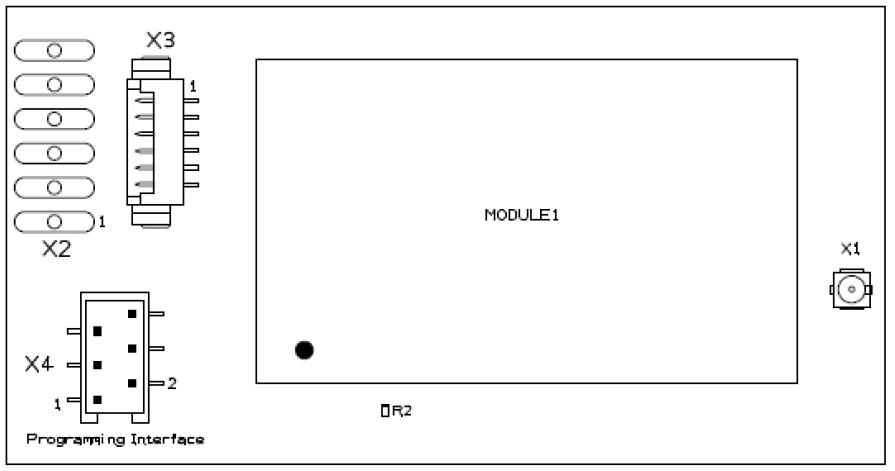
\includegraphics[width=0.8\textwidth]{module.png}
  \caption{overview of the Swarmbee module }
  \label{module}
\end{figure}

\begin{figure}[H]
  \centering
      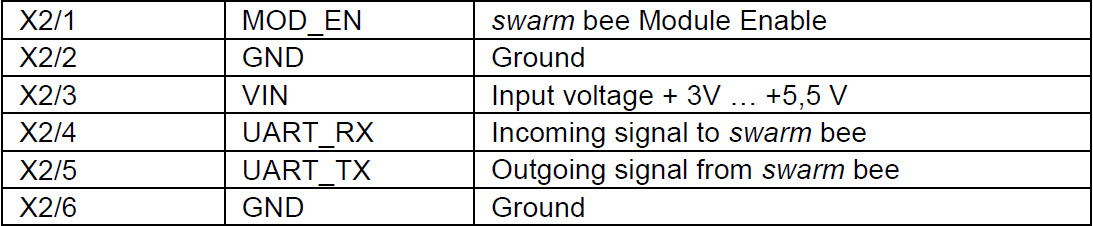
\includegraphics[width=0.8\textwidth]{table.png}
  \caption{Pinout table of the Swarmbee module}
  \label{table}
\end{figure}


\subsection*{Xmega - Swarmbee}
The Xmega sends request and receive data from the
Swarmbee module. This information is transmitted using the UART protocol.
The communication is mainly used for sending API commands to the Swarmbee
module. The UART connecting uses a baudrate of 115200 bps since this is the
transmission speed of the Swarmbee module. The Xmega uses two pins, RX
(PC2), TX (PC3) to achieve a wired connection with the Swarmbee. For debugging pin PC7 en PC8 are reserved. The debugging connecting can be established with a terminal such as Putty.

\begin{figure}[H]
  \centering
      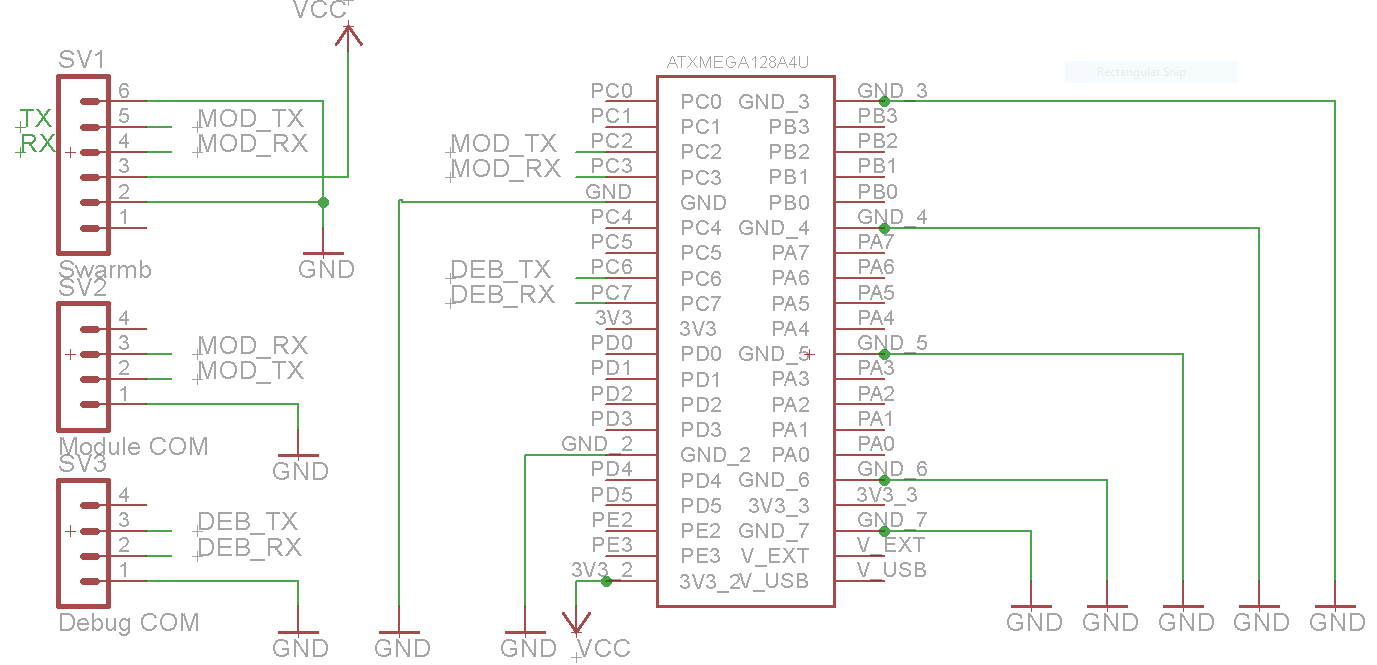
\includegraphics[width=\textwidth]{schema.png}
  \caption{Wiring diagram of the xmega and the Swarmbee module}
  \label{schema}
\end{figure}

Figure \ref{schema} shows the wiring diagram made for a PCB to connect the Xmega with the Swarmbee and to easily connect the two serial ports.


\section*{Software}
In the software we first declare the necessary things like UART initialization and clock speed. To communicate with the swarm bee we use: "command();", to print something to the debug log we use "DebugPrint();". In main.c, the custom message of the ranging request notification is set to 0 because we don't need any extra information at this time, this can be set to your own needs. Also the interval of the broadcast message gets set, these are represented by the following lines:
\lstinputlisting[firstline=7,lastline=8,label=code:id,caption=]{./manual.c}

In the while of main.c, the function "DetermineCommandtype();" gets excecuted when a ranging request notification has been received, this is checked by the function: ValidateMessage(),. If a message is corrupted this will not get trough.
\lstinputlisting[firstline=10,lastline=11,label=code:id,caption=]{./manual.c}

This function can be found in transreceive.c, This is where the incoming messages get decomposed and analysed, character for character. The beginning of each message will be compared to an expected order of characters, this can be extended with any kind of expected message. When the received string starts with "*RRN", we know that the string can be used be used to fill the population list, function: "fillpopulationlist();" will be executed.
\lstinputlisting[firstline=13,lastline=14,label=code:id,caption=]{./manual.c}

In the function "fillpopulationlist.c" the information from the received notification get seperated by the commas between the values. this function uses the functions from list.c to fill the dynamic array. The following functions are included in list.c:

    \begin{itemize}
        \item PrintHeaderList(); This function prints the static information of the list.
        \item print\_list(); This funtion prints the dynamic information of the list.
        \item append(); The append function fills the list from the end of the list.
        \item insert(); The insert function fills the list from the beginning of the list.
        \item popListByNumber(); Finds and replaces data by the index numbers of the list.
        \item popListByValue(); Finds and replaces data by the list variable to be found.
        \item sizeOfList(); Returns the size of the total list.
    \end{itemize}

When a ranging request of 5 nodes has filled the dynamic array, the populationlist will look like follow:
\begin{figure}[H]
  \centering
      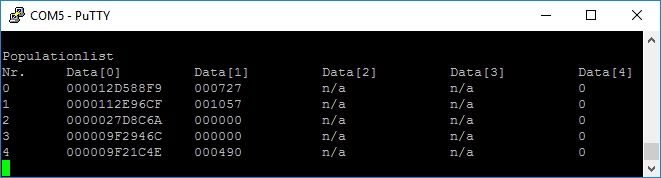
\includegraphics[width=\textwidth]{populationlist.png}
  \caption{Putty log of the filled population list}
  \label{list}
\end{figure}

%----------------------------------------------------------------------------------------
%	BIBLIOGRAPHY
%----------------------------------------------------------------------------------------

\bibliographystyle{unsrt}

\bibliography{sample}

%----------------------------------------------------------------------------------------

\end{document}